%!TEX root = ../report.tex

\begin{document}
    \chapter{Introduction}

%-------------------------------------------------------------------------------
%	Motivation
%-------------------------------------------------------------------------------
    \section{Motivation}
    
        Every day people are exposed to have some kind of accident and the worst kind of accidents are those that put their lives at risk.
        Fortunately, for those kinds of accidents, we have rescue services like firefighters.
        But firefighters are humans and put their lives at risk trying to save other lives.
        According to the Deutscher Feuerwehrverband (German Firefighters Association), the number of firefighters missions in Germany in 2017 
        ascends to more than 3 million, and the number of deaths in fires in 2016 was approximately 350 \cite{DeutscherFeuerweherverband_online}.
        \par
        What if the firefighters are supported by rescue robots?
        With the use of rescue robots that explore the accident areas, we can help firefighters do their job more safely.
        Rescue robots can explore buildings to find entrances, exits, and other key areas that help the firefighters to rescue people in a faster and efficient way.
        But robots cannot find their exact position inside a building with a single GPS, because this kind of technology is unreliable under certain conditions 
        (e.g. inside buildings).
        \par
        In this work, we try to enable rescue robots to explore buildings with the use of LiDAR systems and 3D models of the buildings.
        With the use of LiDAR systems, we can obtain representations of the actual status of buildings at risk without endangering any lives. 
        These kinds of representations are known as point clouds.
        With the use of CityGML models \cite{Groger_2012_OGC}, we have access to the 3D representation of many buildings in Germany.
        Using modern registration techniques, one can find a match between the point cloud given by the LiDAR system and the 3D model of the building.
        The registration result can be then used to find the exact position of the robot with respect to the building.
        The registration result can also help to locate relevant parts of the building like windows, doors, stairs, or corridors.
        This information can be presented to the firefighters in a way that enables them to elaborate on a rescue plan, with the only objective of 
        supporting firefighters in their mission to rescue lives and safeguard theirs.

%-------------------------------------------------------------------------------
%	Challenges and Difficulties
%-------------------------------------------------------------------------------
    \section{Challenges and Difficulties}
    
        Most of the registration algorithms are focused on working for two point clouds.
        Just a few registration algorithms address the registration of 3D models with point clouds.
        And between those registration algorithms, only a couple are created to work with CityGML models, as described in \autoref{chap:State of the Art}.
        \par      
        The registration process is normally done manually, due to the fact that it is a simple task for a human since we all learn to match patterns when we are just kids. 
        The automation of registration is complicated because for a computer it is difficult to find features and match them between two different types of 3D data.
        \par
        An additional challenge is the data itself, the point clouds available are partial and they do not represent the whole 3D model, 
        normally they just capture part of the walls of the buildings and the surface outside the buildings.
        And vice versa, the 3D models do not have information of the surface outside the buildings.
        The only information available in both, the 3D models and the point cloud, are some of the walls of the buildings.
        \par
        At the time this work was started, there was no GPS information of the point clouds used in the registration, just of the CityGML model. 
        Therefore, it was not possible to perform a coarse registration with GPS information and the coarse registration need to be done by other means.
        Moreover, there was just one test set available for the evaluation of the solution.
        All this together made deciding on a specific approach difficult.
        \par

%-------------------------------------------------------------------------------
%	Problem Statement
%-------------------------------------------------------------------------------
    \section{Problem Statement}
        This work intends to implement an automated registration method for a point cloud with a CityGML model.
        This automated registration method will then be used as part of the A-DRZ (Aufbau des Deutschen Rettungsrobotik-Zentrums) project of the Fraunhofer IAIS.
        Figure \ref{fig:adrz} shows the system architecture of the A-DRZ project. 
        The final objective of the automated registration in the A-DRZ project is to be able to look inside the CityGML models, in order to 
        find the location and status of relevant parts of the buildings (e.g. doors, windows, stairs, and corridors) that can be used for rescue task.

        \begin{figure}[H]
            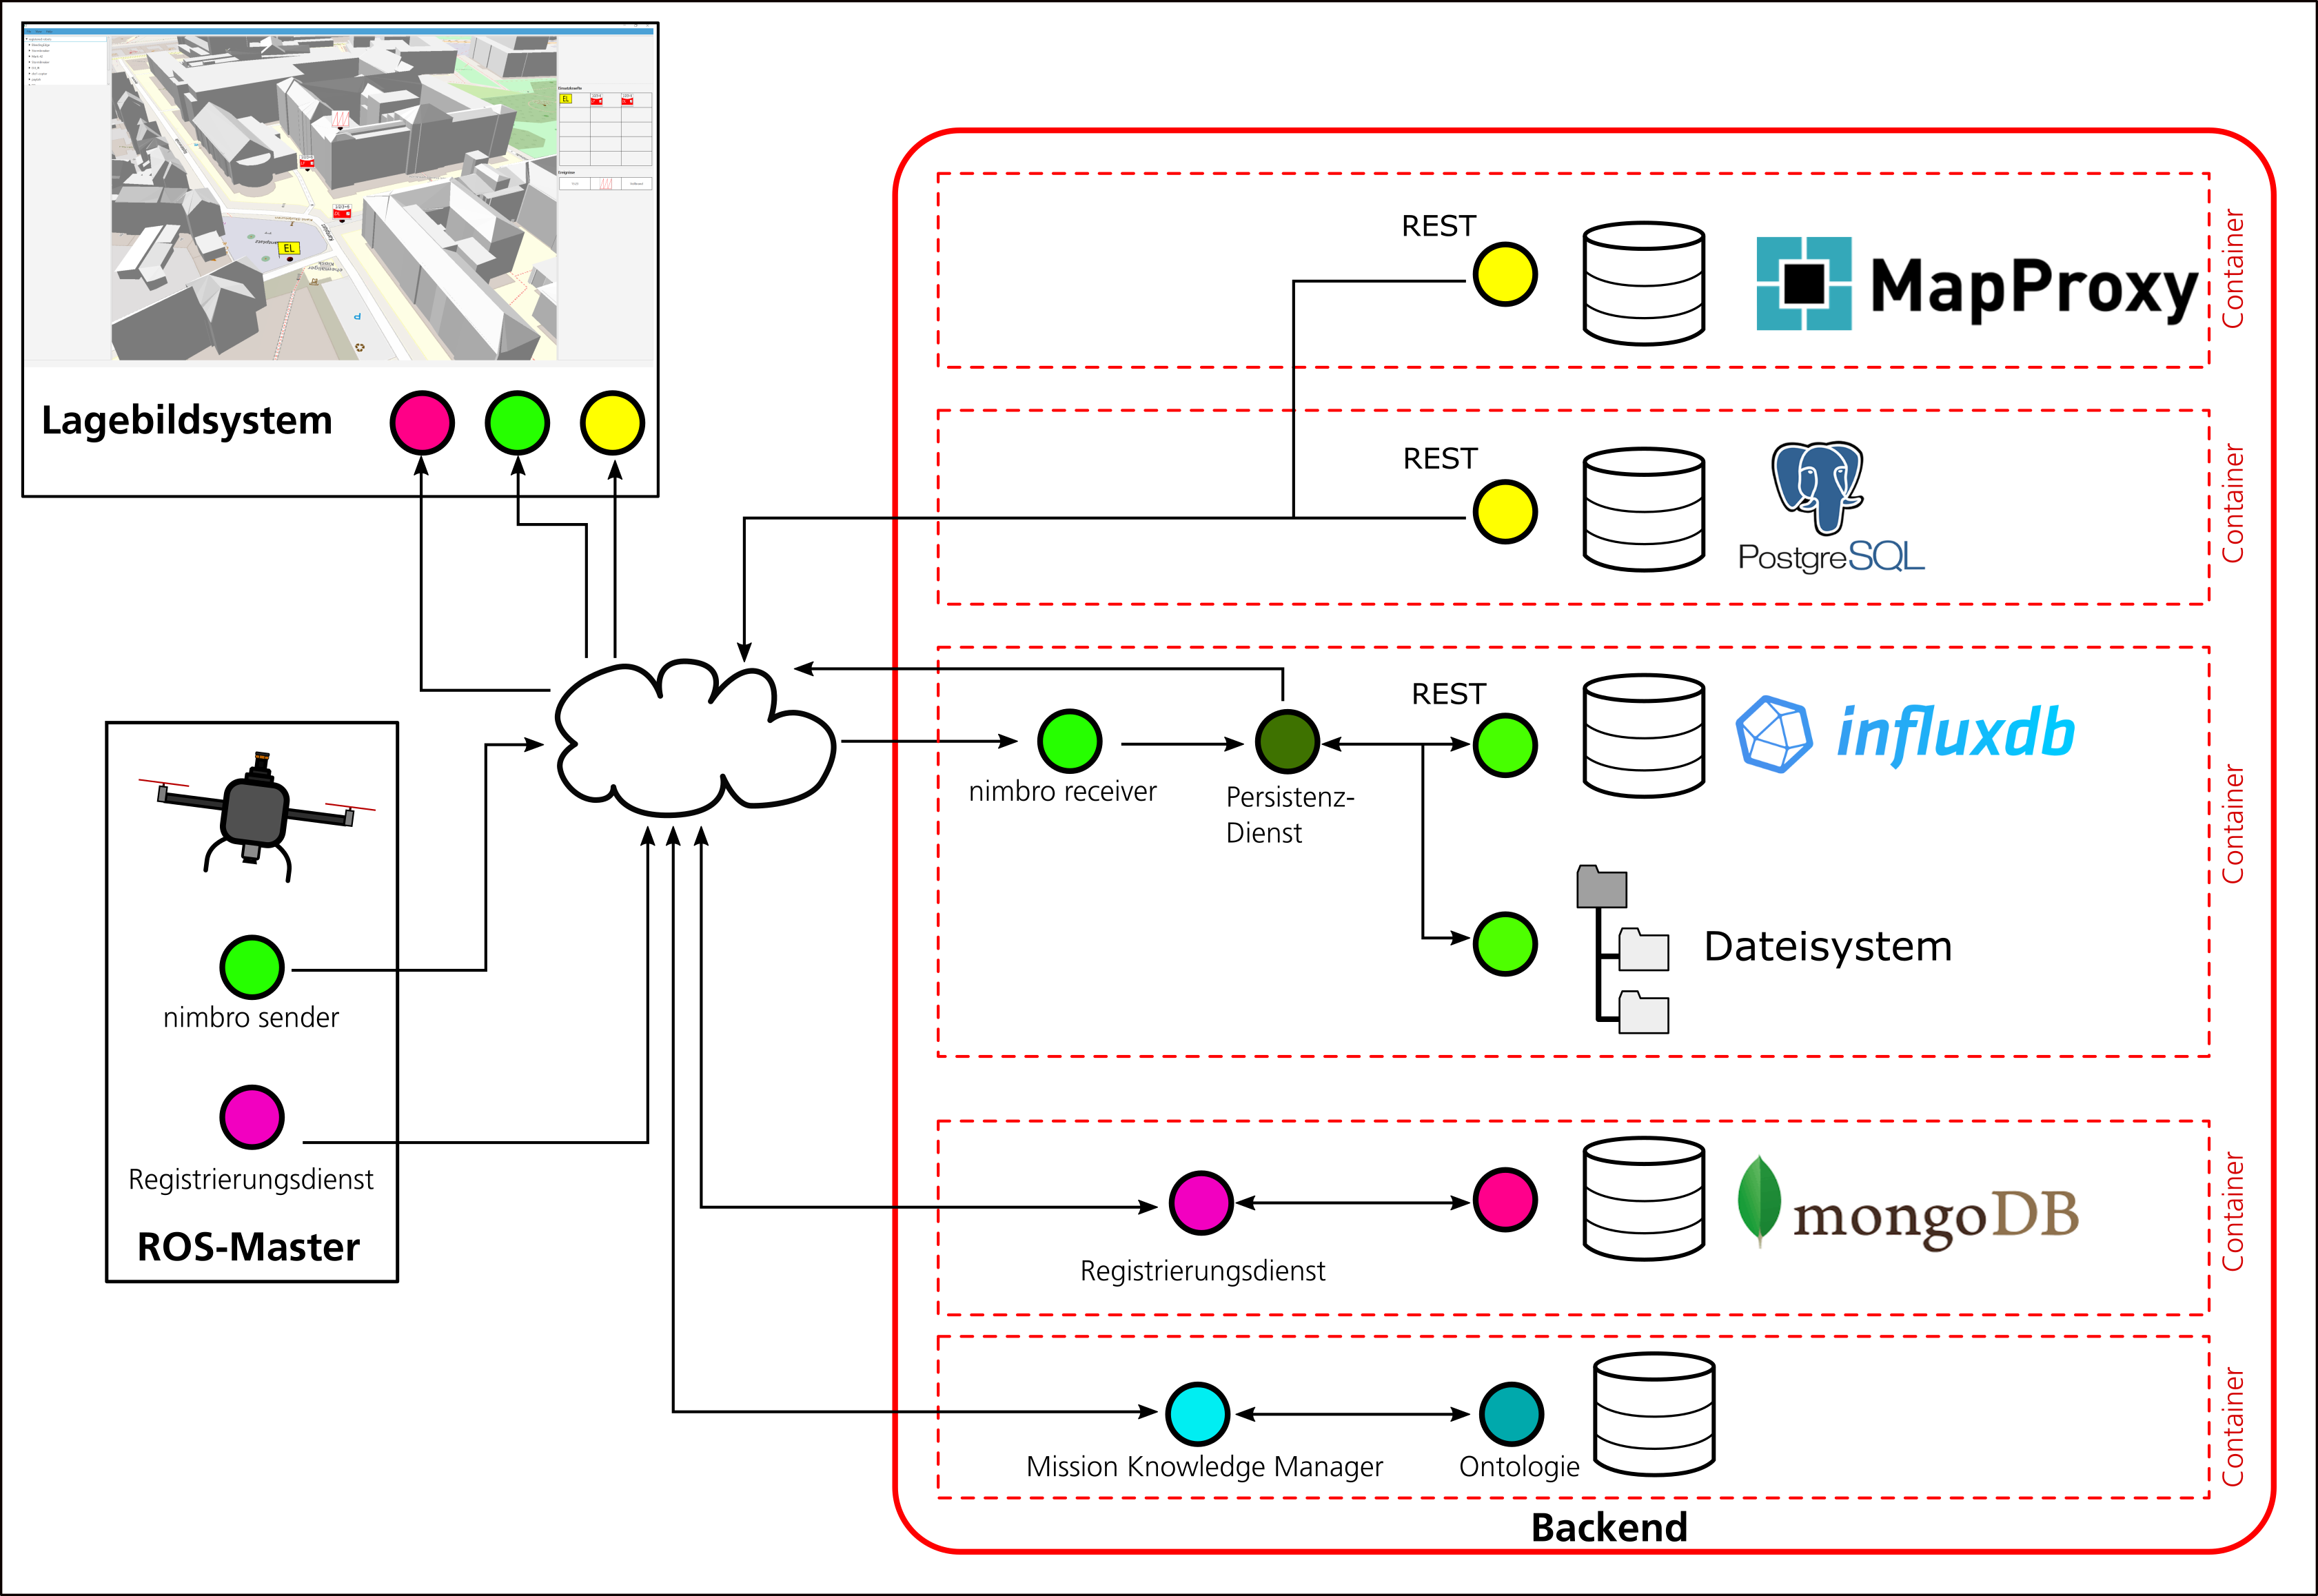
\includegraphics[width=\textwidth]{images/Systemaufbau.png}
            \caption{A-DRZ architecture system.}
            \label{fig:adrz}
        \end{figure}

        The current automated approaches are mainly focused on point-to-point registration.
        Therefore, the exploration of point-to-model automated registration methods is necessary to implement a solution that aims to work in real-time.
        Moreover, there is no automated process implemented in A-DRZ project yet. 
        However, as an assistance system, the A-DRZ project should avoid human interaction for performing the registration.

        Figure \ref{fig:system_diagram} shows the general workflow of the needed method.
        The input of the method is a point cloud together with the corresponding CityGML model of a building  
        (the process to obtain this is outside of the scope of this work).
        The provided input is then preprocessed and used for the registration algorithm.
        The output of the registration algorithm is a transformation that maps the point cloud to the CityGML model.
        Finally, the output transformation and the input data are used for visualization of the point cloud on the CityGML model.

        \begin{figure}[H]
            \centering
            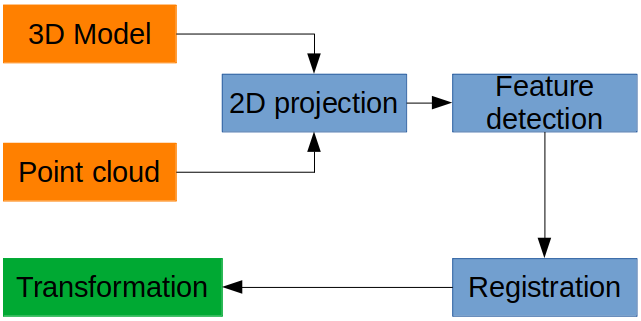
\includegraphics[scale=0.5]{images/RegistrationProcess}
            \caption{System diagram.}
            \label{fig:system_diagram}
        \end{figure}

        Firstly, the implementation will be tested individually.
        Secondly, the implementation will be tested with its integration on a visualization software of the Fraunhofer IAIS.
        This visualization software is a simple 3D rendering of CityGML models limited to a certain geographical area.
        Thirdly, the implementation will be tested with its integration on the A-DRZ project.


\end{document}
